\chapter[Introdução]{Introdução}

A música eletrônica e a cultura \textit{DJ} têm desempenhado um papel essencial na transformação do cenário musical contemporâneo, desde o surgimento dos primeiros equipamentos de mixagem nos anos 70 até os sofisticados sistemas digitais da atualidade. A figura do \textit{DJ}, em sua origem limitada a um curador de faixas, evoluiu para um artista completo, que utiliza a tecnologia para manipular sons em tempo real, criando experiências sonoras únicas e imersivas. No centro dessa transformação está o \textit{mixer}, que, ao longo das décadas, se tornou uma ferramenta indispensável para performances, permitindo a combinação de múltiplos canais de áudio em uma nova e coesa composição musical.

A evolução dos equipamentos de mixagem, no entanto, não explorou as formas de compreensão de uma faixa, de forma que o entendimento da composição de uma música permanece constante desde a criação dos primeiros equipamentos, baseado no controle de ganho em 3 filtros passa-bandas. Embora as inovações tecnológicas tenham ampliado a quantidade de canais, a integração com telas digitais e a conectividade em nuvem, a lógica básica da mixagem permanece rígida, muitas vezes limitando o potencial criativo dos artistas. Atualmente, muitos DJs enfrentam desafios para personalizar suas performances de forma mais orgânica e adaptativa, sendo obrigados a trabalhar dentro das limitações dos sistemas disponíveis.

\begin{figure}[h]
    \centering
    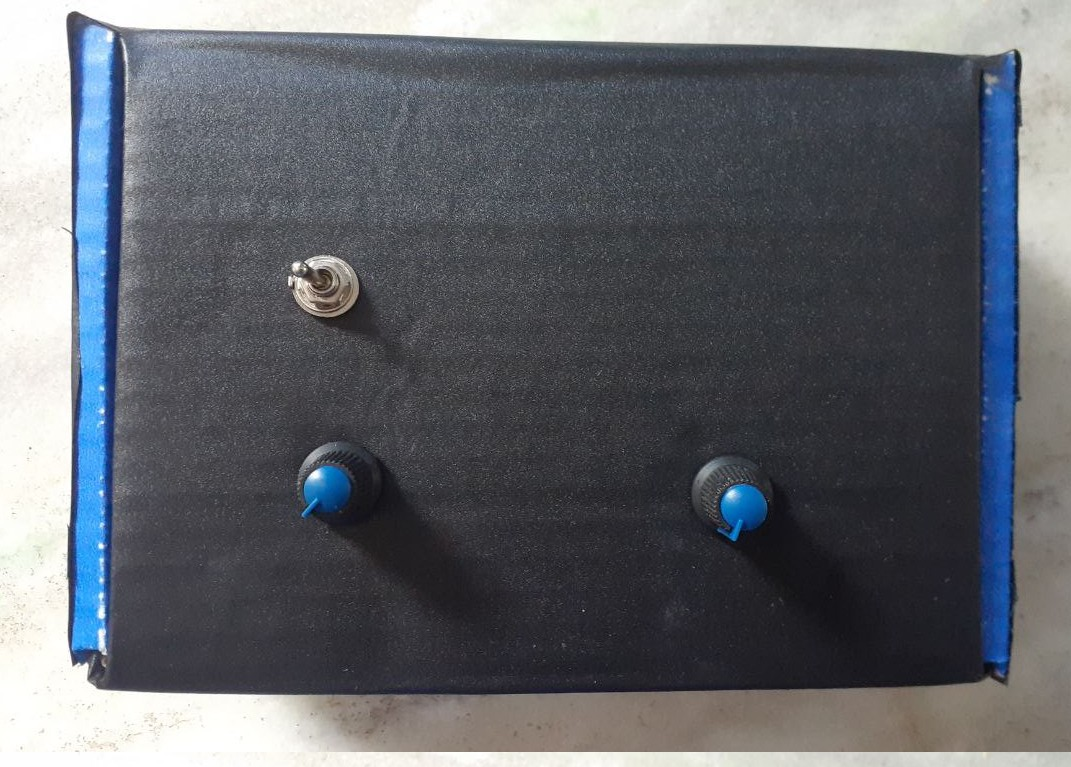
\includegraphics[width=0.5\textwidth]{figuras/fig97.jpg}
    \caption{Protótipo de \textit{mixer}}
    \label{fig97}
\end{figure}

Neste cenário, surge a necessidade de uma abordagem que não apenas expanda as possibilidades técnicas, mas também permita uma maior flexibilidade no controle e manipulação dos elementos sonoros. O presente projeto visa justamente explorar novas formas de explorações e controle no processo de mixagem, desenvolvendo um protótipo de \textit{mixer} que se adapte de maneira mais natural às necessidades dos profissionais. Com o foco em oferecer uma otimização da forma como uma transição é feita, o protótipo, presenta na Figura tal, propõe um \textit{mixer} que unifica a forma de controle sob os canais, tradicionalmente conhecida pelo ganho em três bandas por canal, ao utilizar filtro passa-altas que deslizam ao longo de toda a banda, para que o controle dos elementos sonoros, ao invés de três botões por canal, utilize um, de forma que ambos canais sejam controlados de forma unificada, promovendo assim um novo paradigma de como se pensar a mixagem na cultura \textit{DJ}.

\section{Justificativa}
O mercado de equipamentos para \textit{DJs} é amplamente dominado por grandes empresas, mas existe uma crescente demanda por dispositivos que fogem à norma estabelecida. Nesse contexto, surgem pequenas empresas e \textit{boutiques} especializadas que desenvolvem soluções inovadoras, atendendo a \textit{DJs} que buscam mais controle criativo e flexibilidade em suas performances. Percebe-se que há uma necessidade crescente de equipamentos que ofereçam mais versatilidade e personalização, permitindo aos \textit{DJs} explorar suas habilidades de forma mais livre, mantendo, no entanto, a praticidade e aplicabilidade. A solução proposta busca responder a essa demanda por novos recursos, oferecendo uma abordagem simples e funcional, que se adapta facilmente ao uso cotidiano de um \textit{DJ}.

Através da análise do processo de transição entre faixas, observou-se que os \textit{mixers} tradicionais funcionam com a manipulação independente dos controles de frequências para cada canal. A transição típica envolve a diminuição dos graves de uma faixa, enquanto aumenta-se os elementos agudos da próxima faixa, de modo a suavizar a mudança diferentes elementos para que não haja uma variação brusca nos elementos. Ao perceber esse padrão de manipulação, surgiu a ideia de unificar os controles, permitindo um controle mais intuitivo e direto, sem perder a capacidade de personalização.

Com essa unificação, a solução proposta modifica o conceito tradicional de controle de frequências. Em vez de ajustar bandas de frequência separadamente, a ideia é utilizar um controle único de corte de frequências, que atuaria de forma simultânea nos dois canais, permitindo uma transição mais fluida e simplificada. Essa abordagem não só facilita o trabalho do \textit{DJ}, mas também oferece uma nova maneira de explorar as possibilidades sonoras durante a performance. Essa inovação visa, portanto, ampliar as opções criativas disponíveis de forma que possa ser facilmente aplicável a um sistema atual. 

\section{Objetivos}

Nessa seção, o objetivo geral e os objetivos específicos almejados por esse projeto são citados.

\subsection{Objetivo Geral}
Esse projeto visa a criação de um \textit{mixer} implementado em um sistema embarcado que unifique o controle da mixagem feita por \textit{DJ}s em contrapartida ao modelo tradicional de mixagem baseado em equalização de três bandas.

\subsection{Objetivos Específicos}

Quanto aos objetivos específicos, elencou-se pontos ao longo do desenvolvimento desse sistemas que servirão como pontos de referência para garantir que o funcionamento do todo. 

\begin{enumerate}
    \item \label{item:deslocamento} Realizar de forma automatizada o controle da frequência de corte de dois canais a partir de um controle
    \item \label{item:efeitos} Implementar dois tipos de efeitos: \textit{delay} e \textit{reverb}
    \item \label{item:conversao} Converter o sinal obtido após o processamento para analógico para ser reproduzido por um sistema de som
\end{enumerate}

O Objetivo Específico \ref{item:deslocamento} envolve a obtenção dos sinais de controle, conversões de analógico para digitais, a atuação correta nos filtros passa-altas de ambos canais.

Em relação aos efeitos, o Objetivo Específico \ref{item:efeitos} visa embarcar desde a concepção matemática, implementação do código para cada efeito e sua implementação para que o efeito seja aplicado ao sinal.

Uma vez que a conclusão dos Objetivos acima garante um sinal processado no domínio digital, é necessário garantir que o sinal seja adequadamente convertido para analógico, a fim de ser reproduzido em equipamentos externos. Portanto, o Objetivo Específico \ref{item:conversao} agrega a conversão do sinal de saída para que o sistema de som conectado ao sistema consiga reproduzir o canal de saída.

\section{Estrutura do Documento}

O presente trabalho está organizado em capítulos que abordam os diferentes aspectos da história, desenvolvimento e implementação do protótipo de \textit{mixer} para \textit{DJs} com controle unificado de frequência. A seguir, é apresentada a estrutura do documento.

% O primeiro capítulo, \textbf{Introdução}, faz um delineamento do contexto no qual surgiu a demanda por novas abordagens. Nele, há uma descrição sobre o mercado de equipamentos focados em \textit{DJs} e uma breve explicação sobre como a mixagem é realizada e como esse processo pode ser automatizado. Em seguida, são apresentados os objetivos geral e específicos que guiarão as etapas subsequentes, seguidos de uma descrição sobre a estrutura do texto, detalhando o que cada capítulo aborda para garantir um documento coeso.
No segundo capítulo, \textbf{Fundamentação Teórica e Estado da Arte}, são explorados os conceitos físicos e matemáticos fundamentais, como sinais e sistemas nos domínios contínuo e discreto, % transformações matemáticas e conceitos essenciais para a transição entre os mundos analógico e digital, fundamentais para o tratamento dos sinais provenientes do mundo analógico, que precisam ser convertidos novamente para esse formato. Em seguida, são apresentadas explicações teóricas sobre funcionalidades como filtragem. O capítulo continua explorando
bem como o som, tanto do ponto de vista físico quanto da percepção humana dessa grandeza. Também é realizada uma pesquisa histórica sobre a evolução da mixagem e dos dispositivos utilizados, oferecendo uma compreensão sobre a magnitude e a atuação de um \textit{DJ}, culminando nas formas contemporâneas de mixagem.
% Ainda no segundo capítulo, é detalhada a maneira como o som é trabalhado, destacando como os sinais podem ser compreendidos a partir de duas bandas e como esse parâmetro se relaciona com os elementos que compõem uma música. Além disso, uma pesquisa técnica sobre as conexões entre dispositivos é apresentada, a fim de consolidar a forma como um dispositivo pode interagir com o mundo real.
% Em seguida, 

No terceiro capítulo, \textbf{Metodologia}, a proposta do projeto é descrita a partir de requisitos funcionais e não-funcionais, %, conceitos emprestados da engenharia de \textit{software}. O capítulo se divide 
em duas grandes subseções: prova de conceito e proposta de implementação.
Na prova de conceito, a proposta foi testada utilizando um \textit{software} chamado \textit{PureData}, no qual a lógica de filtragem e efeitos, bem como suas interações, foram implementadas. % Diagramas e descrições detalhadas de cada etapa do processamento são apresentados.
Na proposta de implementação, a solução final é explorada com o detalhamento dos componentes eletrônicos e da solução \textit{software} utilizados.

Para validar tanto a prova de conceito quanto a proposta de implementação, o capítulo \textbf{Resultados} analisa os sinais obtidos a partir da variação dos parâmetros de entrada, de modo a validar o comportamento do sistema para além da simples escuta do sinal final gerado. %Para isso, gráficos no domínio do tempo e da frequência foram utilizados. Com esses resultados, foi possível validar o bom funcionamento da configuração dos filtros utilizados, bem como dos efeitos implementados.

Com o projeto implementado, o capítulo \textbf{Conclusão} realiza uma visão geral de todo o trabalho, destacando a integração de todas as etapas que compuseram o projeto. %Nessa seção, a implementação de um sistema que propõe a alteração e unificação do sistema de mixagem tradicionalmente utilizado pela indústria foi validada por meio da análise dos resultados obtidos.